
 \documentclass[final,3p,times,twocolumn]{elsarticle}

\makeatletter
\def\ps@pprintTitle{%
   \let\@oddhead\@empty
   \let\@evenhead\@empty
   \def\@oddfoot{\reset@font\hfil\thepage\hfil}
   \let\@evenfoot\@oddfoot
}
\makeatother

%% Use the option review to obtain double line spacing
%% \documentclass[preprint,review,12pt]{elsarticle}

%% Use the options 1p,twocolumn; 3p; 3p,twocolumn; 5p; or 5p,twocolumn
%% for a journal layout:
%% \documentclass[final,1p,times]{elsarticle}
%% \documentclass[final,1p,times,twocolumn]{elsarticle}
%% \documentclass[final,3p,times]{elsarticle}
%% \documentclass[final,3p,times,twocolumn]{elsarticle}
%% \documentclass[final,5p,times]{elsarticle}
%% \documentclass[final,5p,times,twocolumn]{elsarticle}

%% The graphicx package provides the includegraphics command.
\usepackage{graphicx}
%% The amssymb package provides various useful mathematical symbols
\usepackage{amssymb}
%% The amsthm package provides extended theorem environments
\usepackage{amsthm}
\usepackage{amsmath}

%% natbib.sty is loaded by default. However, natbib options can be
%% provided with \biboptions{...} command. Following options are
%% valid:

%%   round  -  round parentheses are used (default)
%%   square -  square brackets are used   [option]
%%   curly  -  curly braces are used      {option}
%%   angle  -  angle brackets are used    <option>
%%   semicolon  -  multiple citations separated by semi-colon
%%   colon  - same as semicolon, an earlier confusion
%%   comma  -  separated by comma
%%   numbers-  selects numerical citations
%%   super  -  numerical citations as superscripts
%%   sort   -  sorts multiple citations according to order in ref. list
%%   sort&compress   -  like sort, but also compresses numerical citations
%%   compress - compresses without sorting
%%
%% \biboptions{comma,round}

% \biboptions{}

%\journal{Journal Name}

\begin{document}

\begin{frontmatter}

%% Title, authors and addresses

\title{\huge{New macroprudential regulation and monetary policy in a low interest-rate environment}}

%% use the tnoteref command within \title for footnotes;
%% use the tnotetext command for the associated footnote;
%% use the fnref command within \author or \address for footnotes;
%% use the fntext command for the associated footnote;
%% use the corref command within \author for corresponding author footnotes;
%% use the cortext command for the associated footnote;
%% use the ead command for the email address,
%% and the form \ead[url] for the home page:
%%
%% \title{Title\tnoteref{label1}}
%% \tnotetext[label1]{}
%% \author{Name\corref{cor1}\fnref{label2}}
%% \ead{email address}
%% \ead[url]{home page}
%% \fntext[label2]{}
%% \cortext[cor1]{}
%% \address{Address\fnref{label3}}
%% \fntext[label3]{}


%% use optional labels to link authors explicitly to addresses:
%% \author[label1,label2]{<author name>}
%% \address[label1]{<address>}
%% \address[label2]{<address>}

%\author{\large{ID: 4335707, ID: 4336567, ID: 4341282}}


\begin{abstract}
The aim of this paper is to examine the interaction between the new compulsory capital requirement (CRR) regulation from Basel III, loan-to-value ratio (LTV) regulation, and monetary policy in a low interest-rate environment. In order to do so, we use a dynamic stochastic general equilibrium (DSGE) model which features a housing market, borrowers, savers and banks. For the purpose of understanding how monetary policy complements the new regulation, we compare two different models. Accordingly, our baseline model does not include a role for monetary policy. We then extend this model and consider a standard New Keynesian model with housing market and banking system. For each model, we compare the dynamics after a productivity shock under the new minimum required capital implied by the Basel III framework, and under a higher capital requirement discretionarily set by the regulator. We find that the interaction of monetary policy with relatively strong macroprudential regulation contributes to achieve financial stability, especially in the housing market.

%restrictions on borriwng high m and on amound to lend high CRR strongly contribute to achieve financial stability, especially in the housing market.
%Impulse Response analysis indicate that the interaction of monetary policy aggresive
%banks are constrained the amount they can lend so...

\end{abstract}

\begin{keyword}
macroprudential \sep capital requirement ratio \sep Basel III \sep low interest rate \sep bank regulation
%% keywords here, in the form: keyword \sep keyword

%% MSC codes here, in the form: \MSC code \sep code
%% or \MSC[2008] code \sep code (2000 is the default)

\end{keyword}

\end{frontmatter}

%%
%% Start line numbering here if you want
%%

%% main text
\section{Introduction}
\label{S:1}

%In the last decade: \\ \\

%1) rise of macroprudential policies and tighter financial regulation. \\
%2) steady decline in interest rates supported by unconventional monetary policy. \\ \\

%This paper aims to describe how Basel III regulation (CRR) and LTV macroprudential policy interacts with monetary policy in a low interest rates environment. \\ \\

%Why is this important? Many countries use more than one macroprudential policy, and also have active monetary policy, so policymakers need to know how all these policies may interact in practice. To our knowledge the interaction of both policies has not been studied before in a low interest rate setting. \\ \\

%Lit review \\ \\

%Explain what we do and resutls \\ \\

%Baseline Model is based on Rubio Carrasco 2017 (which is based in the standard Iacoviello 2005) \\ 

%NK Model is based on Rubio Carrasco 2016, which in turn is based on Iacoviello 2015 (banks) and the standard Iacoviello 2005

The 2008 financial crisis made clear that policymakers lacked mechanisms to deal with the build-up of financial imbalances whose sudden unwinding led to serious macroeconomic consequences. It also evidenced the need to depart from the traditional micro-based approach to financial regulation and to adopt a new set of economic policies to achieve financial stability (Galati and Moessner 2013). Soon after the crisis, both scholars and policymakers thus realized that one of the key factors to prevent future financial imbalances was to broaden the set of tools aimed at enhancing system-wide financial stability. In this regard, macroprudential policies have received extensive attention as means to strengthen regulation and supervision.\par

%Indeed, the term macroprudential was first proposed in a report of the Bank for International Settlements in 1978. In 1979, this term was mentioned again in an unpublished document of the Cooke Committee and the Bank of England. Decades later, in a report by the IMF in 1998 it was the first time that macroprudential regulation was mentioned as a mean of financial system supervision. 

After the global financial crisis, macroprudential regulation has gained much more popularity, and policymakers around the world are currently working on implementing these tools. However, the relevant theoretical models and policy instruments are still being studied and debated. Economies all over the world have begun to incorporate the concept of macroprudential supervision in policy formulation in response to the specific situation of each country, but there are considerable differences in how these policies are implemented among countries. Moreover, the formulation of macroprudential policies involves differences in implementation by policymakers in different fields. On the other hand, the goals to be achieved by different policymakers are different and the interaction of different policies need to be selected in light of the actual economic conditions of each country. Many countries use more than one macroprudential policy and also have active monetary policy. Therefore, it is particularly significant to know how all these policies interact in practice.\par


It is clear that empirical evidence on macroprundential policies is still scant, given that they have been widely adopted only in the last decade. As pointed out by Bean (2012), it may be fair to say that we are still in the Stone Age with respect to the employment of macroprudential policies. In fact, there is still plenty to learn about the appropriate macroprudential tools, their transmission mechanisms, their economic outcomes and their relationship with monetary policy. Further, several possible measures have been investigated, but, in contrast to monetary policy, a primary instrument has not been identified yet (Galati and Moessner 2018).\par


Although more analysis is needed, several studies have started to fill this gap. DSGE models are particularly attractive to investigate macroprudential policies, given that this approach is suitable for quantitative experiments, so it has the potential to study the impact of new policy instruments and to provide evidence-based advice to policymakers. This approach suffered sharp critiques after the crisis though, mainly because these models implicitly assumed that financial markets were not subject to frictions (i.e. the Modigliani-Miller theorem holds) and that defaults either do not occur or are exogenous. Since the crisis, however, much effort has been undertaken to address the shortcomings of DSGE models. In fact, these models have offered many insights to the policy debate on macroprudential instruments.

On the lender side, perhaps one of the most popular borrower-targeted tools have been caps on LTV ratios aimed at restricting mortgage lending (Galati and Moessner 2018). In fact, LTV ratios have been widely used by advanced economies as macroprudential tools (Cerutti et al., 2015). In the context of DSGE models, following the seminal work by Kiyotaki and Moore (1997), a stream of studies have surged which introduce limits to borrowing, and some of them incorporate time-varying rules for LTV (e.g. Rubio and Carrasco-Gallego 2014, 2015).\par

On the borrower side, the package of measures from Basel III, which was developed by the Basel Committee on Banking Supervision at the Bank for International Settlements (BIS), introduces new tools to avoid periods of excessive credit growth which can originate severe financial crisis. In particular, this approach consists of two main pillars. The first one considers introducing a mandatory capital conservation buffer of 2.5\%, which combined with the existing minimum capital requirement from Basel II of 8\% yields a required total capital of 10.5\%.\par

The second pillar of Basel III contemplates a countercyclical capital buffer up to another 2.5\% of capital. This measure is designed, in the first place, to help to lean against the build-up phase of the credit cycle, and, in the second place, to reduce the risk that the supply of credit will be constrained by regulatory capital requirements that could undermine the performance of the real economy and result in additional credit losses in the banking system. Moreover, this regulation also incorporates a discretionary element whereby national authorities can implement a buffer of more than 2.5\% if they judge this as appropriate in their national context (BIS, 2015).\par

The aim of the paper is to examine the interaction between the new compulsory capital requirement ratio (CRR) regulation from Basel III, loan-to-value ratio (LTV) regulation, and monetary policy in a low-interest rate environment. In order to do that, we use a dynamic stochastic general equilibrium (DSGE) model which features a housing market, borrowers, savers and banks. In particular, we are interested in analyzing two different scenarios for capital regulation. The first one is a "normal-times" scenario in which the total required capital is at its maximum level without considering the countercyclical buffer (10.5\%). The second one is an "exuberance" scenario in which the regulator decides to set the capital buffer in a way that the total required capital is 20\%.\par

For the purpose of understanding how monetary policy complements the new Basel III regulation, we compare two different models. Accordingly, our baseline model does not include a role for monetary policy, and it follows the setup adopted by Rubio and Carrasco-Gallego (2017). We then extend this model and consider a role for monetary policy in a standard New Keynesian model, following Rubio and Carrasco-Gallego (2016).\par 

For each model, we compare the dynamics after a productivity shock under the two different scenarios for the CRR, and we also consider different caps on the LTV ratio for each of these two cases. Moreover, since the financial crisis advanced countries find themselves with extraordinarily low interest rates, which are known to be prone to speculative episodes and the emergence of financial bubbles (Baldwin and Teulings, 2014). Therefore, in order to provide insights on macroprudential policy under these new economic circumstances, we calibrate the model in a way to simulate a low-interest rate environment in steady state as in Rubio and Yao (2017). Simulations results indicate that the interaction of monetary policy with aggressive macroprudential regulation contribute to achieve financial stability, especially in the housing market.\par


The rest of the paper is organized as follows, Section 2 reviews the literature, Section 3 describes our baseline setup, Section 4 describes our New Keynesian setup, Section 5 presents the results of the simulations for these two models, and Section 6 concludes.\par


\section{Literature Review}

From the perspective of the effectiveness of macroprudential policies, Kannan et al. (2012) constructed a dynamic stochastic general equilibrium (DSGE) model that includes the real estate market. The results of the study show that LTV rule can help maintain financial stability in the face of financial shocks or housing demand shocks. Zhang and Tressel (2017) also assess the effectiveness of macroprudential policies but using a panel VAR model and not a DSGE model. Apart from evaluating the effectiveness of macroprudential policy under the limitation on LTV, a capital requirement ratio (CRR) was introduced, and it was found that it performed well in responding to demand and financial shocks. However, it was slightly worse in response to supply shocks (Angelini et al., 2011).\par

Although the main objective of macroprudential policies is to maintain financial stability, macroprudential policies alone are not sufficient. Scholars have discussed the need for a combination of macroprudential policy and monetary policy. It has been remarked that only when macroprudential policies and monetary policy work together, the objectives of macroprudential supervision can be achieved (Angelini et al., 2011). Unlike this paper, Quint and Rabanal (2014) also point out that the conflict between macroprudential policy and monetary policy is mainly due to a lack of cooperation. In addition, Angelini et al. (2014) study the interaction between capital requirements and monetary policy. The results of the study also showed that the lack of cooperation between macroprudential policies and monetary policies leads to excessive fluctuations in interest rates and capital requirements. Furthermore, Otaviano and Cavallari (2013) point out how monetary policy should integrate macroprudential regulation into traditional monetary policy for the case of developing countries. At the same time, Borio and Shim (2017) emphasize the importance of the adjustment of the monetary policy framework and argued that there is a strong complementarity between monetary policy and macroprudential policy.\par

Thus, Nier and Kang (2016) illustrate the interaction between monetary policy and macroprudential policy and argued that when both policies are actively used, the effectiveness of overall policy will be enhanced when there is only one policy without another support. Simultaneously, it was also believed that there is an interaction between monetary policy and macroprudential policy (Svensson and Lars, 2018). The macroprudential policy affects the financial market. In other words, different LTV would affect the residents' borrowing and housing demand structure in different interest rates and the bank loan interest rate environment (Svensson and Lars, 2018). Suh (2012) discussed the combined use effect and welfare loss of macroprudential and monetary policies under different shocks scenarios based on the BGG-DSGE model under the rational expectations contract. It is claimed that the Nash equilibrium will be equivalent to a consistent equilibrium under certain conditions. However, monetary policy and macroprudential policies will not increase the welfare losses of the society.\par

On the contrary, Rubio and Carrasco-Gallego (2014) obtained the optimal monetary policy and macroprudential policy based on the welfare loss function. It was found that there may be a Nash equilibrium that could not achieve a consistent equilibrium. The combination of the two policies significantly improved welfare and increased the stability of system. Levine and Lima (2015) mainly study the relationship between macroprudential policy and monetary policy under the New Keynesian framework, and found that when macroprudential supervision was introduced into the model, the optimal policy analysis results still showed welfare benefits, even though there is no cooperation between them.\par

Therefore, it seems extremely important to understand the interaction between macroprudential policy and monetary policy. Rubio and Carrasco-Gallego (2017) evaluate the welfare and macroeconomic effects of the new fixed capital requirements in the Basel accords using a Real Business Cycle (RBC) model with a housing market, banks, borrowers, and savers. They found that higher capital requirements imposed by Basel I, II and III decrease both the quantity of borrowing and its variability, producing distributional welfare effects among agents. Moreover, they show that the introduction of a macroprudential rule for the countercyclical capital buffer delivers higher welfare for the society than a situation with no regulation. Rubio and Carrasco-Gallego (2016) extends the model by Rubio and Carrasco-Gallego (2017) and study the interaction between Basel I, II and III regulations with monetary policy. In particular, they propose that the CRR follows a rule that responds to deviations of credit from its steady state, and find that the optimal implementation of this macroprudential rule together with monetary policy brings extra financial stability with respect to Basel I and II. Furthermore, the role of macroprodential tools in a low interest-rate environment was illustrated by Rubio and Yao (2017). They show that tighter macroprudential policies on LTV rule can stabilise financial markets and may help monetary policy to stimulate the economy when interest rates are low.\par

In our paper, we study the interaction between the new compulsory capital requirement ratio (CRR) regulation from Basel III, loan-to-value ratio (LTV) regulation, and monetary policy. We base our model setups in Rubio and Carrasco-Gallego (2016, 2017) in order to include a housing market, banks, borrowers, and savers. However, we differ from these papers in that we consider a low interest-rate environment as in Rubio and Yao (2017). We expect this project may provide insights to policymakers on how the interaction between different policies may help to achieve financial stability when interest rates are low.\par


\section{Baseline Model Setup}

Our baseline model replicates the setup adopted by Rubio and Carrasco-Gallego (2017). In this setup, the economy features savers (patient) and borrowers (impatient), banks and a final goods firm. Households provide labour to final good firms and consume both consumption goods and housing. Households are also constrained in the maximum amount they can borrow from banks, which depends on the LTV. Banks act as financial intermediaries between savers and borrowers, and they are constrained in the maximum amount they can lend to borrowers, which depends on the CRR.

%Simplification of Iacoviello (2015) by Rubio and Carrasco (2017 (BANK CAPITAL REQUIREMENTS AND COLLATERALISED
%LENDING MARKETS)

 \subsection{Savers}

Savers maximise their utility function by choosing consumption, housing, and labour:

$$max \displaystyle E_0 \sum_{t=0}^{\infty}\beta_s^t \Bigg[ log C_{s,t} + j log H_{s,t} - \frac{(N_{s,t})^\eta}{\eta} \Bigg] $$

where $\beta_s \in (0,1)$ is the patient discount factor, $E_0$ is the expectation operator, and $C_{s,t}$, $H_{s,t}$ and $N_{s,t}$ represent consumption, housing stock and working hours, respectively. $1/(\eta-1)$ is the labour supply elasticity , where $\eta>0$. $j>0$ represents the relative weight of housing in the utility function. Savers face the following budget constraint:

\begin{equation}
C_{s,t} + D_t + q_t(H_{s,t} - H_{s,t-1}) = R_{s, t-1}D_{t-1} + W_{s,t}N_{s,t}
\end{equation}

where $D_t$ denotes bank deposits, $R_{s,t}$ is the gross return from deposits, $q_t$ is the price of housing in units of consumption, and $W_{s,t}$ is the wage rate. 

The first order conditions for this optimisation problem are:

\begin{align}
  \frac{1}{C_{s,t}}  &= \beta_s E_t\Bigg( \frac{1}{C_{s,t+1}}R_{s,t} \Bigg) \\
  \frac{q_t}{C_{s,t}}  &= \frac{j}{H_{s,t}} + \beta_s E_t \Bigg( \frac{q_{t+1}}{C_{s,t+1}} \Bigg)  \\
   W_{s,t}  &= (N_{s,t})^{\eta-1} C_{s,t} 
\end{align}

 \subsection{Borrowers}

Borrowers solve the following problem:

$$max \displaystyle E_0 \sum_{t=0}^{\infty}\beta_b^t \Bigg[ log C_{b,t} + j log H_{b,t} - \frac{(N_{b,t})^\eta}{\eta} \Bigg] $$

where $\beta_b \in (0,1)$ is impatient discount factor, subject to the budget constraint and the collateral constraint: 

\begin{align}
C_{b,t} + R_{b,t-1}B_{t-1} + q_t(H_{b,t} - H_{b,t-1}) &= B_t + W_{b,t}N_{b,t} \\
B_t \le E_t \Bigg( \frac{1}{R_{b,t}}m q_{t+1}H_{b,t} \Bigg)
\end{align}

where $B_t$ denotes banks loans and $R_{b,t}$ is the gross interest rate. $m$ can be interpreted as a loan-to-value ratio. The first order conditions in this case are:

\begin{align}
\frac{1}{C_{b,t}} &= \beta_b E_t\Bigg( \frac{1}{C_{b,t+1}}R_{b,t} \Bigg) + \lambda_{b,t} \\
 \frac{q_t}{C_{b,t}} &= \frac{j}{H_{b,t}} + \beta_b E_t \Bigg( \frac{q_{t+1}}{C_{b,t+1}} \Bigg) - \lambda_{b,t} \frac{1}{R_{b,t}}m E_t q_{t+1} \\
W_{b,t} &= (N_{b,t})^{\eta-1} C_{b,t} 
\end{align}

where $\lambda_{b,t}$ denotes the Lagrange multiplier on the borrowing constraint.

 \subsection{Banks}

Banks solve:

$$max \displaystyle E_0 \sum_{t=0}^{\infty}\beta_f^t \bigg[ log C_{f,t} \bigg] $$

where $\beta_f \in (0,1)$ is the banks' discount factor, subject to the budget constraint, the collateral constraint, and the regulatory constraint:

\begin{align} \label{eq:1} 
C_{f,t} + R_{s,t-1}D_{t-1} + B_t = D_t + R_{b,t-1}B_{t-1} \\ 
\frac{B_t-D_t}{B_t} \leq CRR = 1-\gamma
\end{align}

where $B_t-D_t$ can be defined as capital, so the fraction of capital with respect to assets must be larger than $CRR$ (with $\gamma<1$), which is fixed by the regulator. The first order conditions with respect to deposits and loans are:

\begin{align}
 \frac{1-\lambda_{f,t}}{C_{f,t+1}} = \beta_f E_t \Bigg( \frac{1}{C_{f,t}}R_{s,t}\Bigg) \\
 \frac{1-\gamma\lambda_{f,t}}{C_{f,t+1}} = \beta_f E_t \Bigg( \frac{1}{C_{f,t}}R_{b,t}\Bigg)
\end{align}


where  $\lambda_{f,t}$ denotes the Lagrange multiplier on the banks' borrowing constraint.

 \subsection{Firms}

Firms produce the final consumption good and maximise profits subject to the production function by using labour from both types of households:

\begin{align}
max \displaystyle \Pi_t = Y_t - W_{s,t}N_{s,t} - W_{b,t}N_{b,t} \nonumber \\
Y_t = A_t N_{s,t}^\alpha N_{b,t}^{(1-\alpha)}
\end{align}

where $A_t$ represents a technology parameter, and follows an autoregressive process as follows:

\begin{align}
log(A_t) = \rho_A log(A_{t-1}) + u_A
\end{align}

The firms' first order conditions represent the labour-demand equations, which are given as:

\begin{align}
W_{s,t} &= \frac{\alpha Y_t}{N_{s,t}} \\
W_{b,t} &= \frac{(1-\alpha)Y_t}{N_{s,t}} 
\end{align}

 \subsection{Equilibrium}

The total supply of housing is fixed and it is normalised to unity:

\begin{align}
Y_t = C_{s,t} + C_{b,t} + C_{f,t}
\end{align}

The good market clearing condition is:

\begin{align}
H_{s,t} + H_{b,t} = 1 
\end{align}

Equilibrium in financial markets is derived from the borrowing constraint for banks:

\begin{align}
D_t = (1-CRR)B_t 
\end{align}

\section{New Keynesian Model Setup}

The model presented in this section is very similar to our baseline model presented in Section 3, and it is a replication of the setup adopted by Rubio and Carrasco-Gallego (2016). In short, the only difference is that now we consider a role for monetary policy. In order to do that, we introduce intermediate goods firms, which allows us to obtain a New Keynesian Phillips Curve, and a Taylor rule for setting interest rates.



%Explain that now we introduce a role for monetary policy to investigate how macroprudential policies interact with monetary policy....

%Following Rubio and Carrasco-Gallego (2017) (The new financial regulation in Basel III and monetary policy:A macroprudential approach)

 \subsection{Savers}

$$max \displaystyle E_0 \sum_{t=0}^{\infty}\beta_s^t \Bigg[ log C_{s,t} + j log H_{s,t} - \frac{(N_{s,t})^\eta}{\eta} \Bigg] $$

subject to 

\begin{align}
C_{s,t}& + D_t + q_t(H_{s,t} - H_{s,t-1}) = \frac{R_{s, t-1}D_{t-1}}{\pi_t}  + W_{s,t}N_{s,t} \nonumber \\
&+ \frac{X_t-1}{X_t}Y_t
\end{align}

First order conditions:

\begin{align}
  \frac{1}{C_{s,t}}  &= \beta_s E_t\Bigg( \frac{1}{\pi_{t+1}C_{s,t+1}}R_{s,t} \Bigg) \\
  \frac{q_t}{C_{s,t}}  &= \frac{j}{H_{s,t}} + \beta_s E_t \Bigg( \frac{q_{t+1}}{C_{s,t+1}} \Bigg)  \\
   W_{s,t}  &= (N_{s,t})^{\eta-1} C_{s,t} 
\end{align}

 \subsection{Borrowers}

$$max \displaystyle E_0 \sum_{t=0}^{\infty}\beta_b^t \Bigg[ log C_{b,t} + j log H_{b,t} - \frac{(N_{b,t})^\eta}{\eta} \Bigg] $$

subject to

\begin{align}C_{b,t} + \frac{R_{b,t}B_{t-1}}{\pi_{t+1}} &+ q_t(H_{b,t} - H_{b,t-1}) = B_t + W_{b,t}N_{b,t} \\
B_t &\le E_t \Bigg( \frac{1}{R_{b,t}}m q_{t+1}H_{b,t}\pi_{t+1} \Bigg) 
\end{align}

First order conditions:

\begin{align}
\frac{1}{C_{b,t}} &= \beta_b E_t\Bigg( \frac{1}{\pi_{t+1}C_{b,t+1}}R_{b,t+1} \Bigg) + \lambda_{b,t} \\
 \frac{j}{H_{b,t}} &=  E_t\Bigg( \frac{q_t}{C_{b,t}}\Bigg) - \beta_b E_t \Bigg( \frac{q_{t+1}}{C_{b,t+1}} \Bigg) - \lambda_{b,t}  E_t\Bigg(\frac{1}{R_{b,t}}mq_{t+1}\pi_{t+1}\Bigg) \\
W_{b,t} &= (N_{b,t})^{\eta-1} C_{b,t} 
\end{align}

 \subsection{Banks}

$$max \displaystyle E_0 \sum_{t=0}^{\infty}\beta_f^t \bigg[ log C_{f,t}\bigg] $$

subject to

\begin{align}
C_{f,t} + \frac{R_{s,t-1}D_{t-1}}{\pi_t} + B_t &= D_t + \frac{R_{b,t-1}B_{t-1}}{\pi_t} \\ 
\frac{B_t-D_t}{B_t} &\leq CRR = 1-\gamma 
\end{align}

First order conditions:

\begin{align}
\frac{1}{C_{f,t}} &= \beta_f E_t \Bigg( \frac{1}{C_{f,t+1}\pi_{t+1}}R_{s,t}\Bigg) + \lambda_{f,t} \\
\frac{1}{C_{f,t}} &= \beta_f E_t \Bigg( \frac{1}{C_{f,t+1}\pi_{t+1}}R_{b,t}\Bigg) + \gamma\lambda_{f,t} 
\end{align}

 \subsection{Final and Intermediate goods producers}

Following Iacoviello (2005), it is assumed that there are identical final goods producers that operate under perfect competition and flexible prices. Intermediate goods firms operate under a monopolistic competitive market, and they demand labour according to

\begin{align}
W_{s,t} &= \frac{1}{X_t}\alpha\frac{Y_t}{N_{s,t}} \\
W_{b,t} &= \frac{1}{X_t}(1-\alpha)\frac{Y_t}{N_{s,t}}
\end{align}

where $X_t$ denotes the markup, or the inverse of marginal cost. The Calvo price-setting give rise to a standard New Keynesian Phillips curve as follows:

\begin{align}
    \pi_t = \beta_s E_t \pi_{t+1} - \kappa x_t + u_{\pi t}
\end{align}

where $\kappa = (1-\theta)(1-\beta_s \theta)/\theta$ and $u_{\pi t}$ is a normally distributed cost-push shock. This equation relates inflation positively to future inflation and negatively to the markup.

 \subsection{Monetary Policy}
 
 We consider a Taylor rule which responds to inflation and output growth as follows:
 
 \begin{align}
R_{s,t} = (R_{s,t-1})^\rho \bigg((\pi_t)^{(1+\phi_\pi)} (Y_t/Y_{t-1})^{\phi_y} (1/\beta_s)\bigg)^{(1-\rho)} \varepsilon_{Rt},
\end{align}

where $0\leq \rho \leq 1$ is the parameter associated with interest-rate inertia, $\phi_\pi\ge 0$ and $\phi_y \ge 0$ measure the response of interest rates to current inflation and output growth, respectively. $\varepsilon_{Rt}$ is a white noise shock with zero mean and variance $\sigma_\epsilon^2$.

 \subsection{Equilibrium}

As before, the market clearing conditions are

\begin{align}
Y_t = C_{s,t} + C_{b,t} + C_{f,t} \\
H_{s,t} + H_{b,t} = 1 \\
D_t = (1-CRR)B_t 
\end{align}

\section{Simulations}
\label{S:2}


 \subsection{Calibration}
 
 %Explain why we choose these parameters. Most are standard. The only difference is how we set BETAs, since we are imposing a "low interest rate environment". This idea is borrowed from Rubio and Yao (2017).
 
 
Following Rubio and Yao (2017), we create a low-interest rate environment in which the steady-state interest rate is 2\%. This implies that we set $\beta_s = 0.995$, $\beta_b = 0.985$, and $\beta_f = 0.964$. The steady-state weight of housing in the utility function, $j$, is set to 0.1 so the ratio of housing wealth to GDP is 1.40 in steady state as in Iacoviello (2005). $\eta$ is set to 2, so that the labor supply elasticity is 1.16. Following Iacoviello (2005), the labour income share for savers is set to 0.64. We consider $\theta = 0.75$ implying $\kappa = 0.0858$. For the Taylor rule, we use $\rho = 0.8$ to reflect a realistic degree of interest rate smoothing as in McCallum (2001). Following Rubio and Yao (2017), we set $\theta_\pi$ and $\theta_y$ equal 0.5.\par
 

We simulate the response of the two models to a technology shock. We assume that technology, $A_t$ follows an autoregressive process with persistence $\rho = 0.9$ and a normally distributed shock. Finally, as noted before, we simulate the model for two different values of the CRR, 0.105 ("normal-times" scenario) and 0.20 ("exuberance" scenario). We also consider three possible values for the LTV, $m = {0.7, 0.8, 0.9}$. Table 1 presents a summary of the parameter values used for both models.\par
 

 
\begin{table}[htbp]
\footnotesize
\caption{Parameter values} 
\label{tab:my-table}
\begin{tabular}{lll}
\hline
$\beta_s$ & .995       & Discount factor for savers                        \\
$\beta_b$ & .985       & Discount factor for borrowers                     \\
$\beta_f$ & .964       & Discount factor for banks                         \\
$j$       & .1         & Weight of housing in utility function             \\
$\eta$    & 2          & Parameter associated with labour elasticity       \\
$\alpha$  & .64        & Labour income share for savers                    \\
$\theta$  & 0.75       & Probability of not changing prices  \\
$\rho_A$  & .9         & Technology persistence                            \\
$\kappa$  & .0858      & Response of inflation to changes in markup        \\
$\rho$    & .8         & Interest rate smoothing parameter                 \\
$\phi_\pi$ & .5         & Response of interest rate to changes in inflation \\
$\phi_y$  & .5         & Response of interest rate to changes in output    \\
$m$       & .7; .8; .9 & Loan-to-value ratio                               \\
$CRR$     & 0.105; .2  & Capital Requirement Ratio                         \\
\hline
\end{tabular}
\end{table}
 
 
 \begin{figure*}[ht]
\centering
  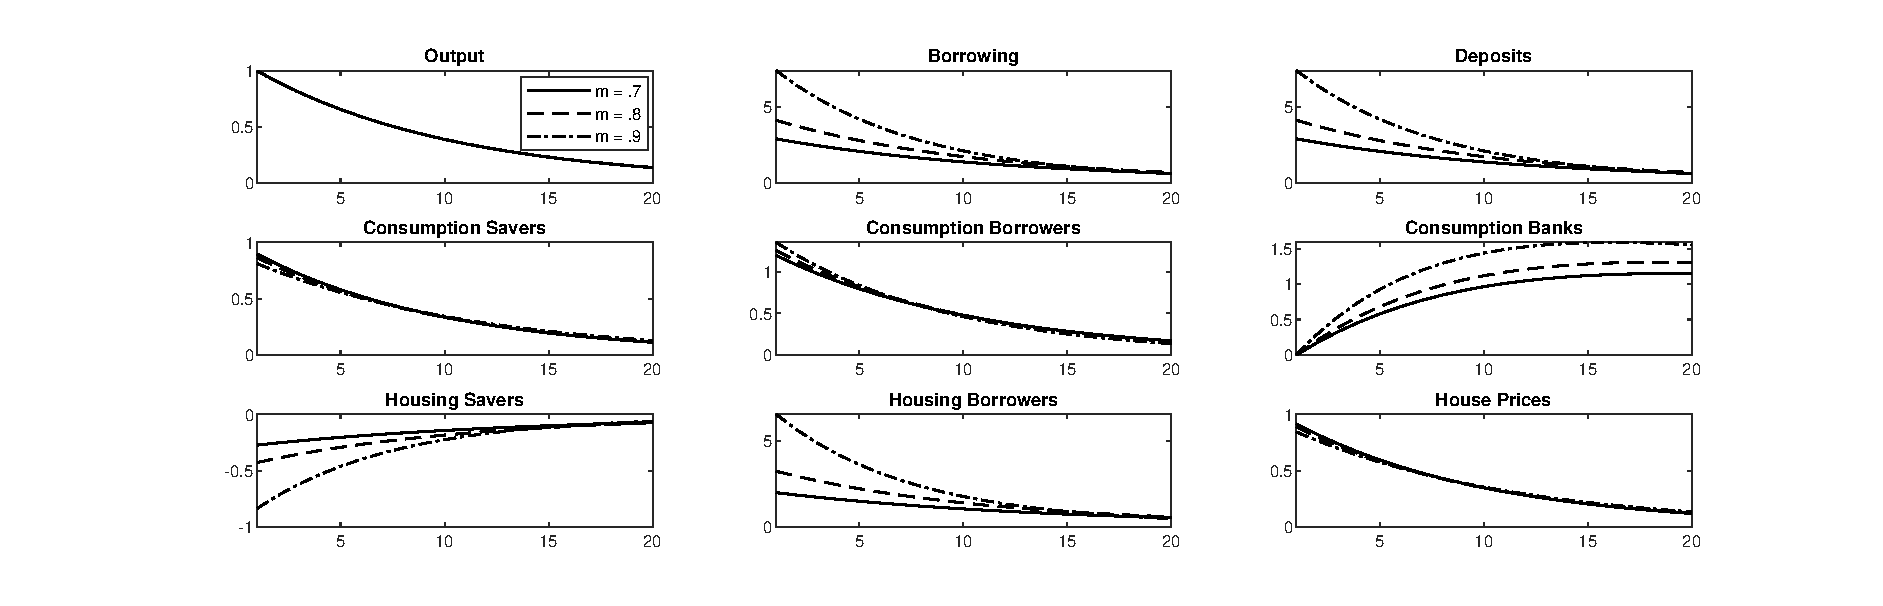
\includegraphics[width=\linewidth]{fig1_rbc_crr_105.eps}
  \caption{Baseline Model. Impulse responses to a technology shock. Different loan-to-values ratios and $CRR=10.5\%$.}
    \label{fig:fig1}
\end{figure*}

  

 \subsection{Dynamics}
 
  \subsubsection{Baseline Model}
  
 Figure \ref{fig:fig1} displays impulse responses to a technology shock in the baseline model with a CRR=10.5\%. In general, the direct effect of the shock is an increase in output, and both savers' and borrowers' consumption. The income increase triggers a raise in borrowers’ housing demand and therefore in borrowing. The rise in house prices is driven mainly by the positive technology shock, as they are not significantly affected by changes in housing demand triggered by tightening the LTV ratio. The fact that savers’ demand for houses decreases (given the rise in their price) and borrowers’ demand increases instead, can be attributed to the relative impatience of borrowers’ (lower $\beta$). Furthermore, borrowers’ consumption increases more that savers’ consumption because the rise in house prices increases the value of their collateral, allowing them to consume more.\par


\begin{figure*}[ht]
\centering
  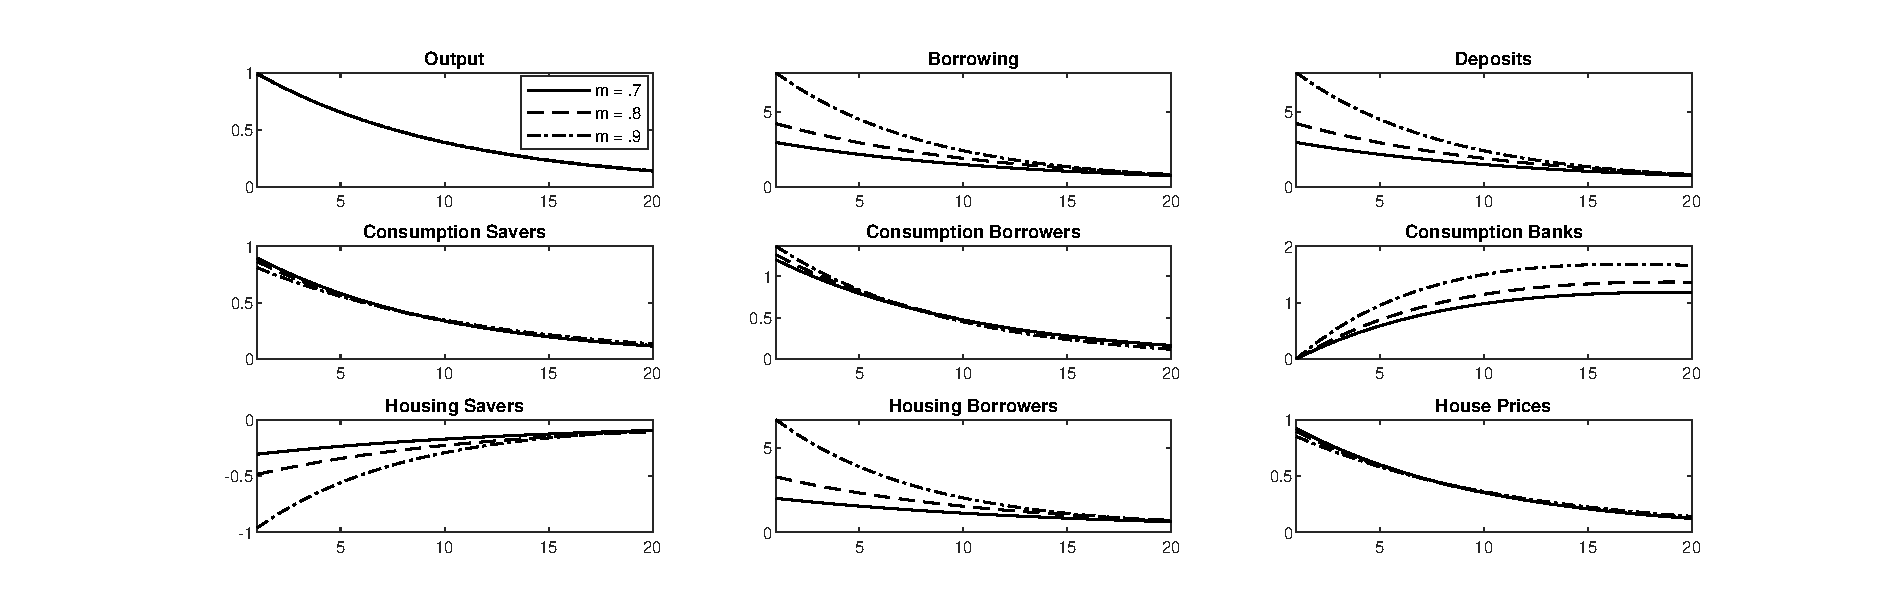
\includegraphics[width=\linewidth]{fig2_rbc_crr_20.eps}
  \caption{Baseline Model. Impulse responses to a technology shock. Different loan-to-values ratios and $CRR=20\%$.}
    \label{fig:fig2}
\end{figure*}


Comparing the differences between different levels of the LTV ratio we can see that a tightening of the constraint unambiguously reduces the magnitude of the impulse responses and, therefore, stabilises the dynamics of the system around the steady state equilibrium. In particular, output and consumption are little changed, as the LTV ratio does not change the direct effects of a supply side shock. However, being borrowers constrained in the amount of credit they can get, borrowing and house demand increase significantly less for tighter values of the LTV, causing also banks’ deposits and consumption to increase by a smaller amount.\par

Figure \ref{fig:fig2} shows the impulse responses in the same framework but CRR=20\%. It is clear that setting a higher capital requirement for banks does not have an evident effect on the dynamics of the model. This result is actually quite predictable, as the main instruments used by banks are interest rates, which are not considered by the benchmark set-up. 
Therefore, while the LTV ratio contributes considerably in stabilising the economy, the CRR is not significantly useful in a framework where monetary policy does not have a role.\par

 
  
\begin{figure*}[ht]
\centering
  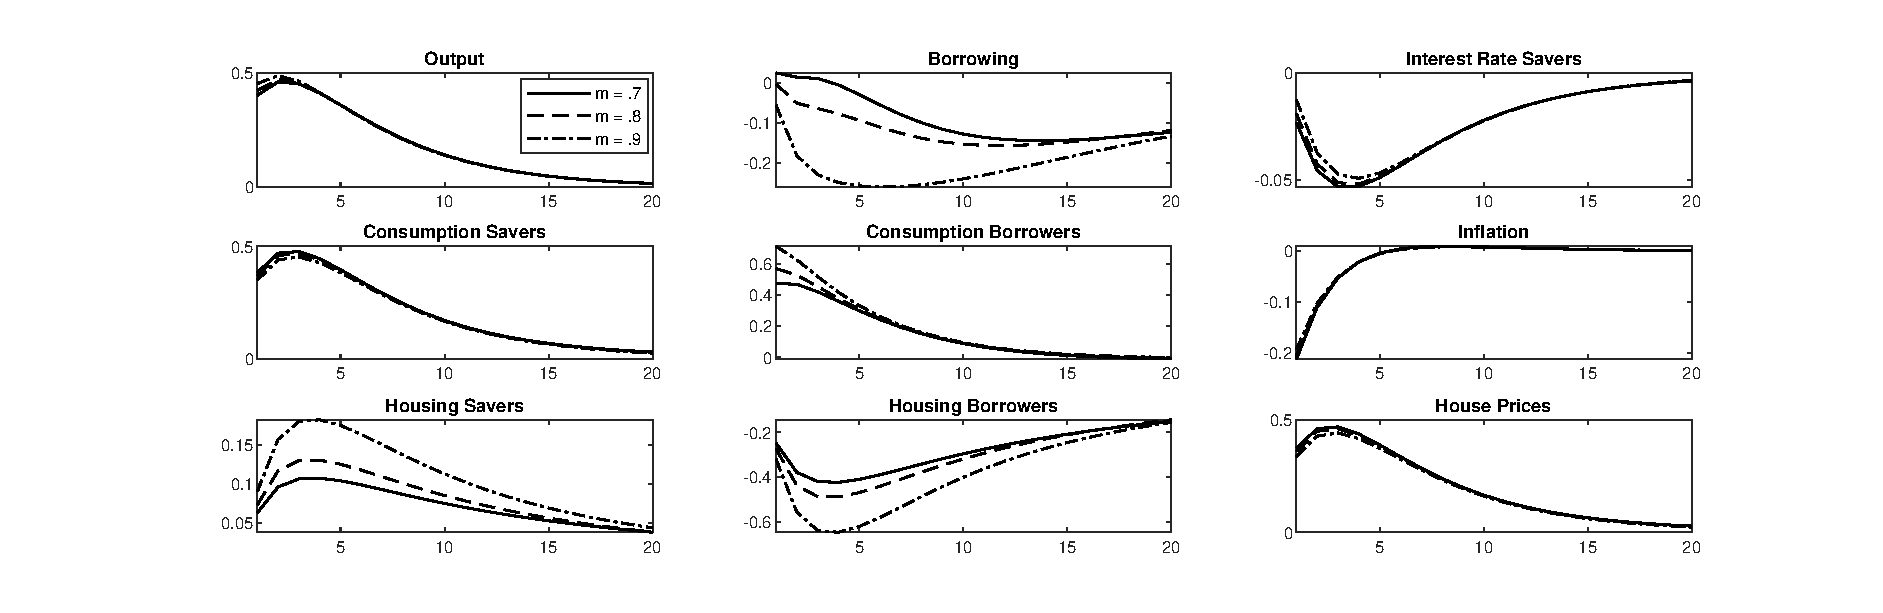
\includegraphics[width=\linewidth]{fig3_nk_crr_105.eps}
  \caption{New Keynesian Model. Impulse responses to a technology shock. Different loan-to-values ratios and $CRR=10.5\%$.}
    \label{fig:fig3}
\end{figure*}


  
   \subsubsection{New Keynesian Model}
 
  Figure \ref{fig:fig3} shows impulse responses to a technology shock in the New Keynesian framework with CRR=10.5\%.
  
First, notice that the introduction of a monetary policy reduces sensibly the magnitude of the fluctuations and the rapidity of the responses (producing hump shaped dynamic paths), as it is already well known. Qualitatively, the effects of the shock are similar to the previous model as regards output, households and bank consumption, house prices and deposits. Inflation and interest rate decrease according to the NKPC.
The difference with the benchmark set-up lies the housing and credit market: the demand for houses is now increasing for savers and decreasing for borrowers, borrowing decreases as well. This might be a sign that the macroprudential mix is too tight, in fact, the aim of the macroprudential policy is to limit fluctuations, not to reduce borrowing per se.\par

\begin{figure*}[ht]
\centering
  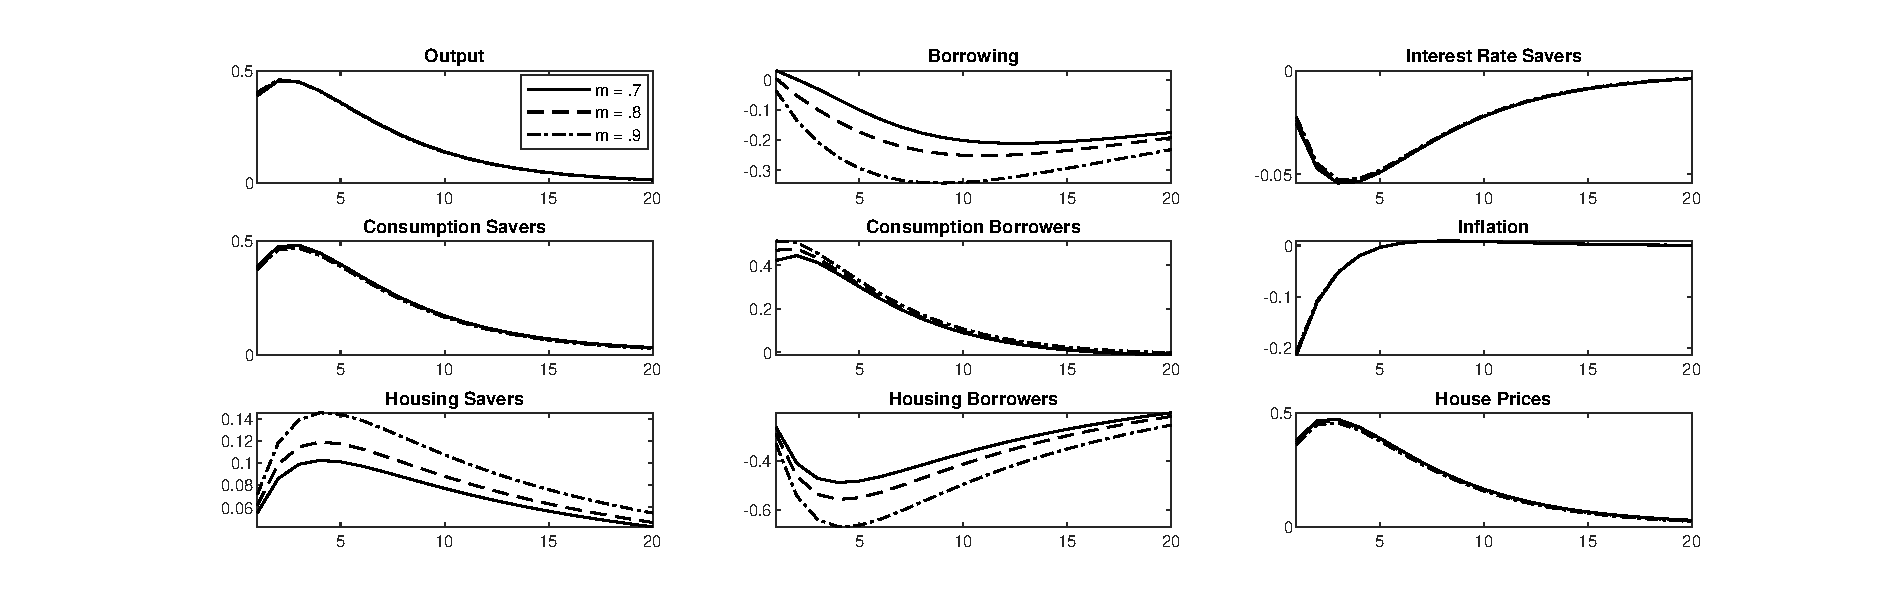
\includegraphics[width=\linewidth]{fig4_nk_crr_20.eps}
  \caption{New Keynesian Model. Impulse responses to a technology shock. Different loan-to-values ratios and $CRR=20\%$.}
    \label{fig:fig4}
\end{figure*}

Now, comparing the different levels of LTV ratio notice that a tighter constraint smooths the response to borrowing and therefore borrowers’ consumption, and the response to housing demand. With higher LTVs, borrowers can get less credit, therefore consume less goods and houses. Overall, the increase in the LTV ratio reduces the volatility in credit and housing markets, at the cost of slightly bigger volatility in the interest rate.\par

Figure \ref{fig:fig4} shows impulse responses to a technology shock in a NK framework with CRR=20\%.
Qualitatively, the responses are the same as the previous case. However, the magnitude of the responses of consumption and housing demand are weakened. This happens because a tighter constraint affects the amount of credit that banks issue, as it is clear from comparing the impulse response for credit in figures \ref{fig:fig3} and \ref{fig:fig4}. It is interesting to notice that the stabilising power of the CRR rule is higher when the LTV ratio constraint is looser, i.e. the more one macroprudential policy stabilises the system, the less will the other one be effective (notice that the response of interest rate is much less affected by changes in the LTV ratio when switching from a 10.5\% to a 20\% CRR). Therefore we can say that an additional instrument is useful when the current instruments are not too limiting.\par

\section{Concluding remarks}

The paper analyses qualitatively the interaction between monetary policy and two different macroprudential constraints, namely a LTV ratio and a CRR on banks, and their effects on the business cycle in a low-interest rate environment. To do so, we construct two different general equilibrium models, one RBC with housing market, banks and financial frictions, and a NK model with housing and banks as in Rubio and Carrasco (2016). We then obtain impulse responses for a standard calibration and different levels of the two macroprudential constraints in order to observe the dynamics of the main economic variables.\par

We find that, in both frameworks, a tighter LTV ratio increases sensibly the stability of the system, and when a role for monetary policy is specified, the stabilising effect of the LTV ratio is weaker because the monetary rule itself has a stabilising role. As regards the CRR we observe no significant contribution of a rise in the ratio on the dynamics of the business cycle. That is because the interest rate, which is the main instrument through which banks operate, does not have a role in the baseline framework. In the New Keynesian set-up, on the contrary, a rise in the CRR reduces the volatility of the main real variables, even though the effect of the policy is weaker as the LTV ratio is tighter. However, if both constraint are too tight, credit might undesirably fall during an economic expansion, it is then necessary to carefully choose the right combination of macroprudential policies. Therefore, an additional instrument can be useful when the existing policy is not too limiting and especially when it cannot be tightened due to information asymmetries or political instability.
A shortcoming of the paper is that the analysis provided is purely qualitative and an interesting addition would be a quantitative analysis of the optimal macroprudential policy combination. \par


%\section{Discussion}
%\label{S:3}
 % Comment how dynamics change in NK Model vs Baseline Model. In other words, what different does monetary policy make.


 \section*{References}
 
Angelini, P., Neri, S., \& Panetta, F. (2011). Monetary and macroprudential policies. Bank of Italy Temi di Discussione (Working Paper) No, 801. \\

Angelini, P., Neri, S., \& Panetta, F. (2014). The interaction between capital requirements and monetary policy. Journal of money, credit and Banking, 46(6), 1073-1112. \\

Baldwin, R., \& Teulings, C. (2014). Secular stagnation: facts, causes and cures. London: Centre for Economic Policy Research-CEPR. \\ 
 
Bank for International Settlements (2015). Frequently asked questions on the Basel III Countercyclical Capital Buffer. \\
 
Bean, C. (2012). Central banking in boom and slump. JSG Wilson Lecture in Economics. \\ 

Borio, C. E., \& Shim, I. (2007). What can (macro-) prudential policy do to support monetary policy?, BIS Working Paper, 242. \\

Canuto, O., \& Cavallari, M. (2013). Monetary policy and macroprudential regulation: Whither emerging markets. The World Bank. \\

Cerutti, E., Claessens, S., \& Laeven, L. (2017). The use and effectiveness of macroprudential policies: New evidence. Journal of Financial Stability, 28, 203-224. \\ 

Galati, G., \& Moessner, R. (2013). Macroprudential policy–a literature review. Journal of Economic Surveys, 27(5), 846-878. \\ 

Galati, G., \& Moessner, R. (2018). What do we know about the effects of macroprudential policy?. Economica, 85(340), 735-770. \\ 

Iacoviello, M. (2005). House prices, borrowing constraints, and monetary policy in the business cycle. American economic review, 95(3), 739-764. \\ 

Kannan, P., Rabanal, P., \& Scott, A. M. (2012). Monetary and macroprudential policy rules in a model with house price booms. The BE Journal of Macroeconomics, 12(1). \\

Kiyotaki, N., \& Moore, J. (1997). Credit cycles. Journal of political economy, 105(2), 211-248. \\ 

Levine, P., \& Lima, D. (2015). Policy mandates for macro-prudential and monetary policies in a new Keynesian framework. \\

McCallum, B. T. (2001). Should monetary policy respond strongly to output gaps?. American Economic Review, 91(2), 258-262. \\

Nier, E. W., \& Kang, H. (2016). Monetary and macroprudential policies–exploring interactions. BIS Paper, (86e). \\

Quint, D., \& Rabanal, P. (2014). Monetary and macroprudential policy in an estimated DSGE model of the euro area (No. 2014/5). Diskussionsbeiträge. \\

Rubio, M., \& Carrasco-Gallego, J. A. (2014). Macroprudential and monetary policies: Implications for financial stability and welfare. Journal of Banking \& Finance, 49, 326-336. \\ 

Rubio, M., \& Carrasco‐Gallego, J. A. (2015). Macroprudential and monetary policy rules: a welfare analysis. The Manchester School, 83(2), 127-152. \\ 

Rubio, M., \& Carrasco-Gallego, J. A. (2016). The new financial regulation in Basel III and monetary policy: A macroprudential approach. Journal of Financial Stability, 26, 294-305. \\ 

Rubio, M., \& Carrasco‐Gallego, J. A. (2017). Bank capital requirements and collateralised lending markets. The Manchester School, 85, 79-103. \\ 

Rubio, M., \& Yao, F. (2017). Macroprudential policies in a low interest-rate environment. Reserve Bank of New Zealand Discussion Papers DP2017/04. \\ 

Suh, H. (2012). Macroprudential policy: its effects and relationship to monetary policy. FRB of Philadelphia Working Paper No. 12-28. \\

Svensson \& Lars, E.O (2018). Monetary policy and macroprudential policy: Different and separate?. Canadian Journal of Economics/Revue canadienne d'économique, 51(3), 802-827. \\

Zhang, Y., \& Tressel, T. (2017). Effectiveness and channels of macroprudential policies: lessons from the Euro area. Journal of Financial Regulation and Compliance, 25(3), 271-306. \\

%% The Appendices part is started with the command \appendix;
%% appendix sections are then done as normal sections
%% \appendix

%% \section{}
%% \label{}

%% References
%%
%% Following citation commands can be used in the body text:
%% Usage of \cite is as follows:
%%   \cite{key}          ==>>  [#]
%%   \cite[chap. 2]{key} ==>>  [#, chap. 2]
%%   \citet{key}         ==>>  Author [#]

%% References with bibTeX database:

%\bibliographystyle{model1-num-names}
%\bibliography{sample.bib}

%% Authors are advised to submit their bibtex database files. They are
%% requested to list a bibtex style file in the manuscript if they do
%% not want to use model1-num-names.bst.

%% References without bibTeX database:

% \begin{thebibliography}{00}

%% \bibitem must have the following form:
%%   \bibitem{key}...
%%

% \bibitem{}

% \end{thebibliography}


\end{document}

%%
%% End of file `elsarticle-template-1-num.tex'.